\chapter{Background}
% section 1 : delaunay triangulation
% delauanay property and its incremental construction
\section{Delaunay Triangulation}
Delaunay triangulation is method of triangulation where every simplex obeys delaunay crieteria. In 2D triangulation, if every triangle has empty circumcircle, then it is a delaunay triangulation. Similarly in 3D, if every tetrahedra has empty circumsphere, then it is delaunay. Empty circumcircle condition states that there should not be any point inside or on that circumcircle in 2D or circumsphere in 3D except the points of simplex as shown in Figure \ref{fig:del_tri}.

% some diagrams of delaunay triangulation with empty circumcircle
\begin{figure}[h]
	\centering
	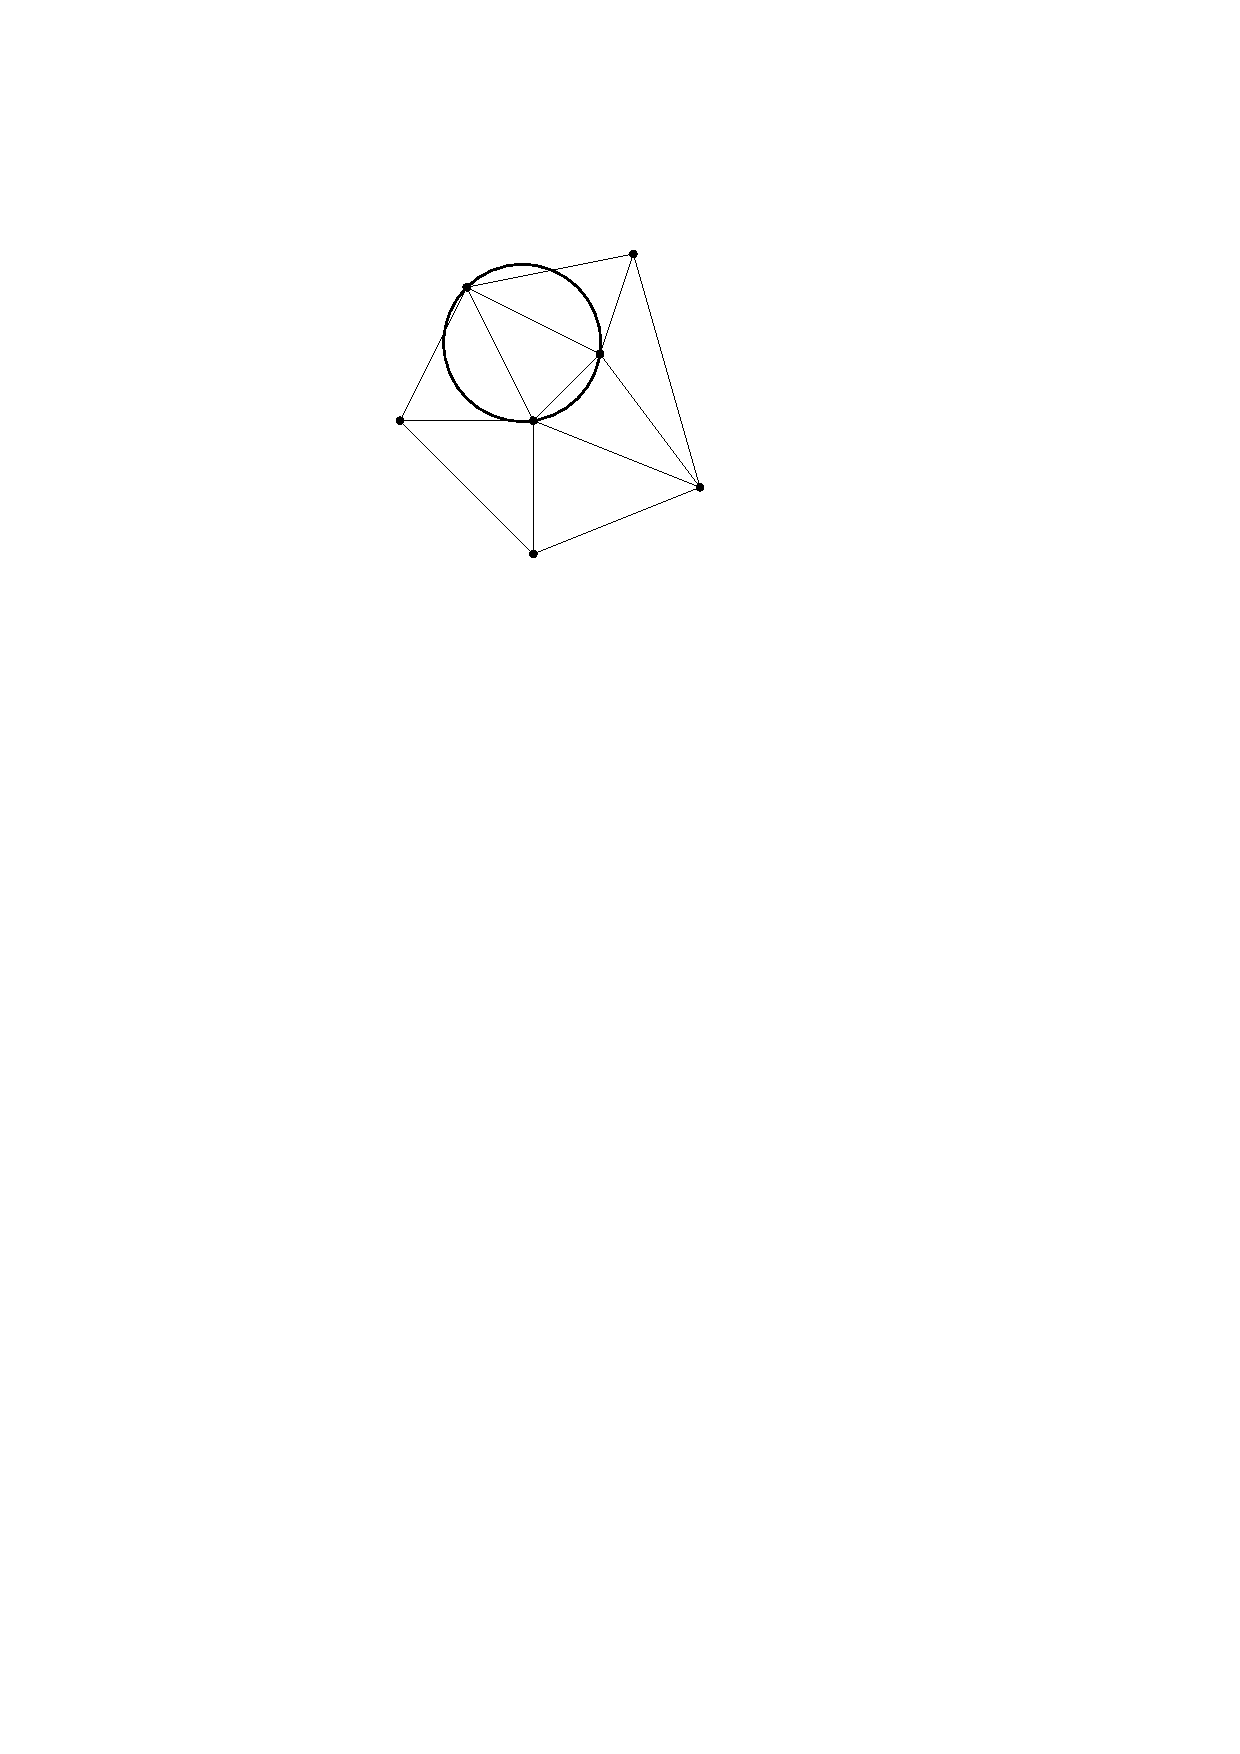
\includegraphics{images/del_tri.pdf}
	\caption{Delaunay triangulation and empty circumcircle}
	\label{fig:del_tri}
\end{figure}

For a point set in general position, there always exists a unique delaunay triangulation. In 2D, points are in general position when there are no set of 4 points such that they all lie on same circle. If they lie on same circle, then there is more than one way to connect those 4 points to form delaunay triangulation as shown in Figure \ref{fig:non_general_pos}. To resolve this ambiguity, perturbation techniques are used.

\begin{figure}[h]
    \centering
    \begin{subfigure}[t]{0.5\textwidth}
        \centering
        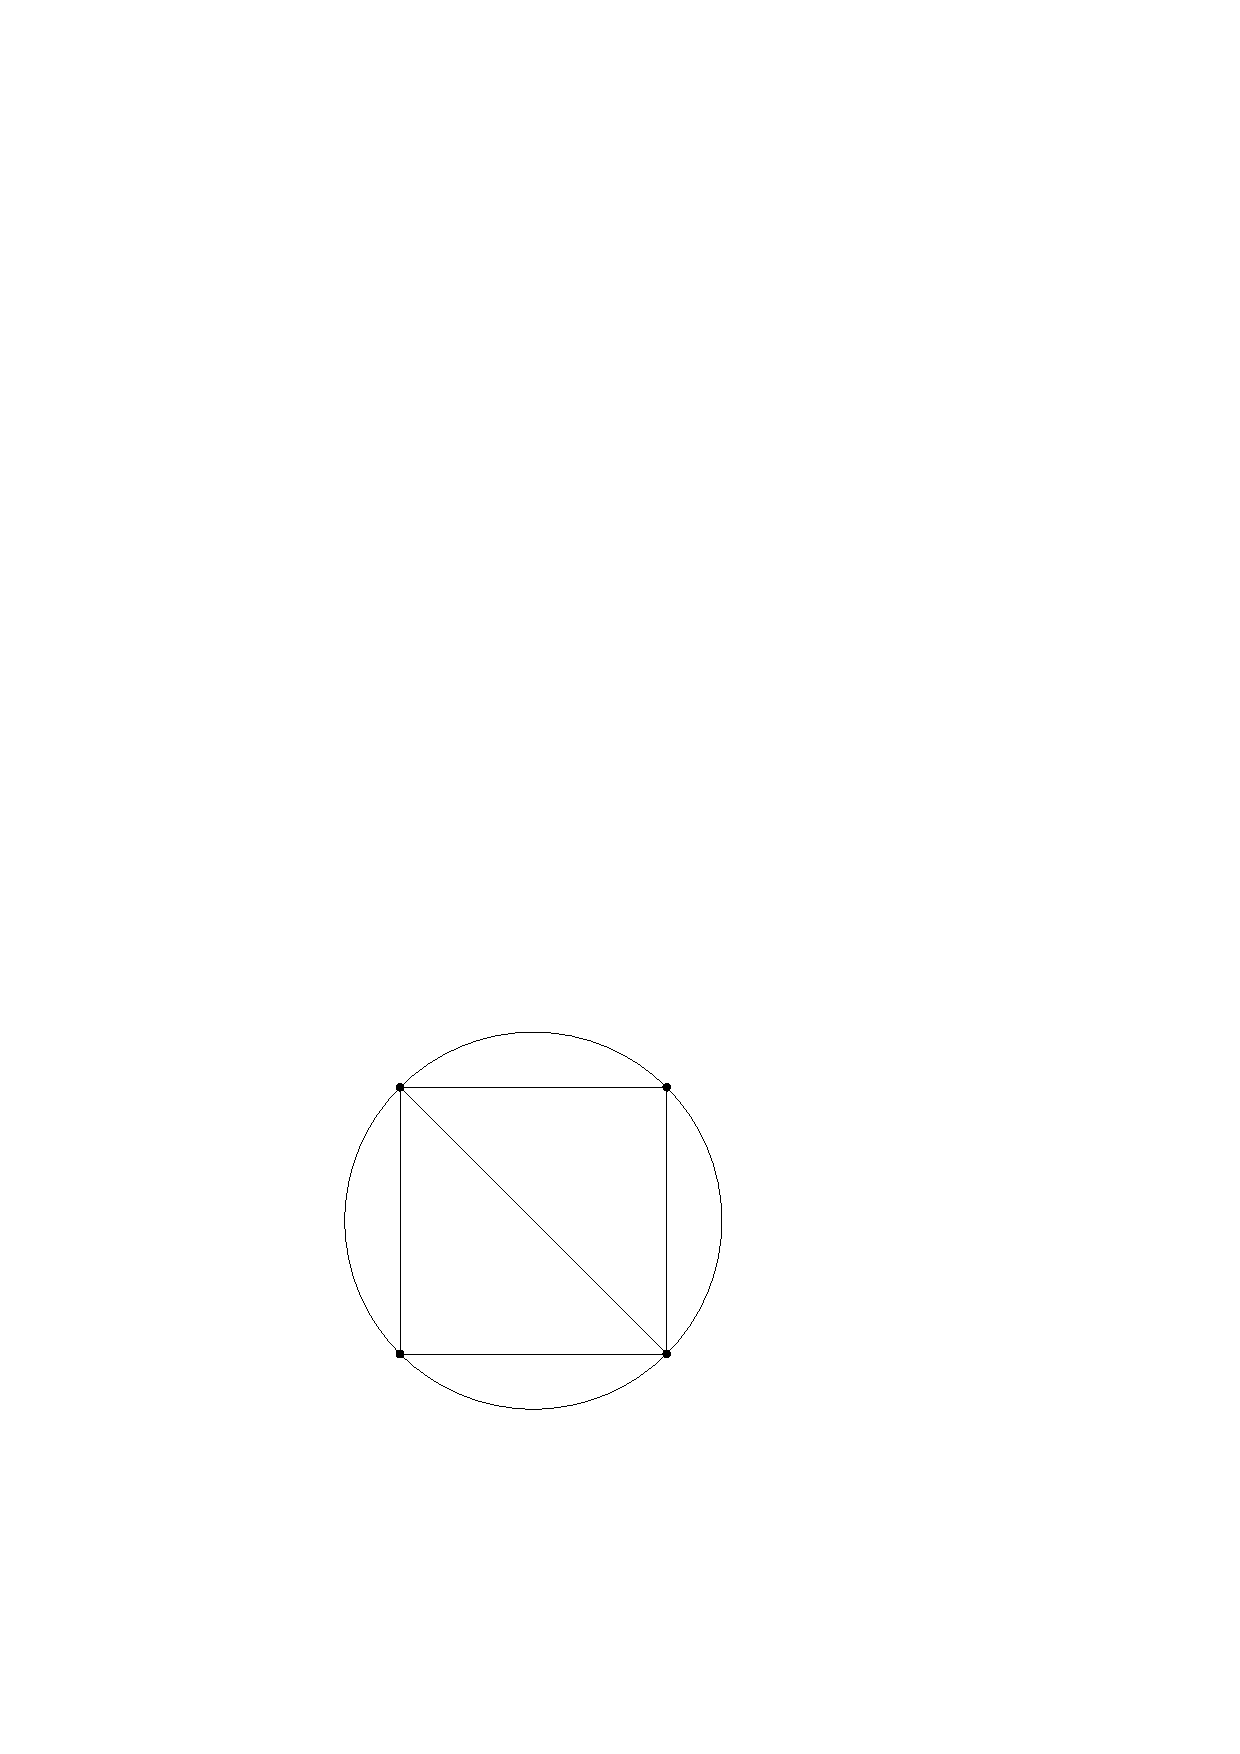
\includegraphics{images/non_general_pos_a.pdf}
    \end{subfigure}%
    \begin{subfigure}[t]{0.5\textwidth}
        \centering
        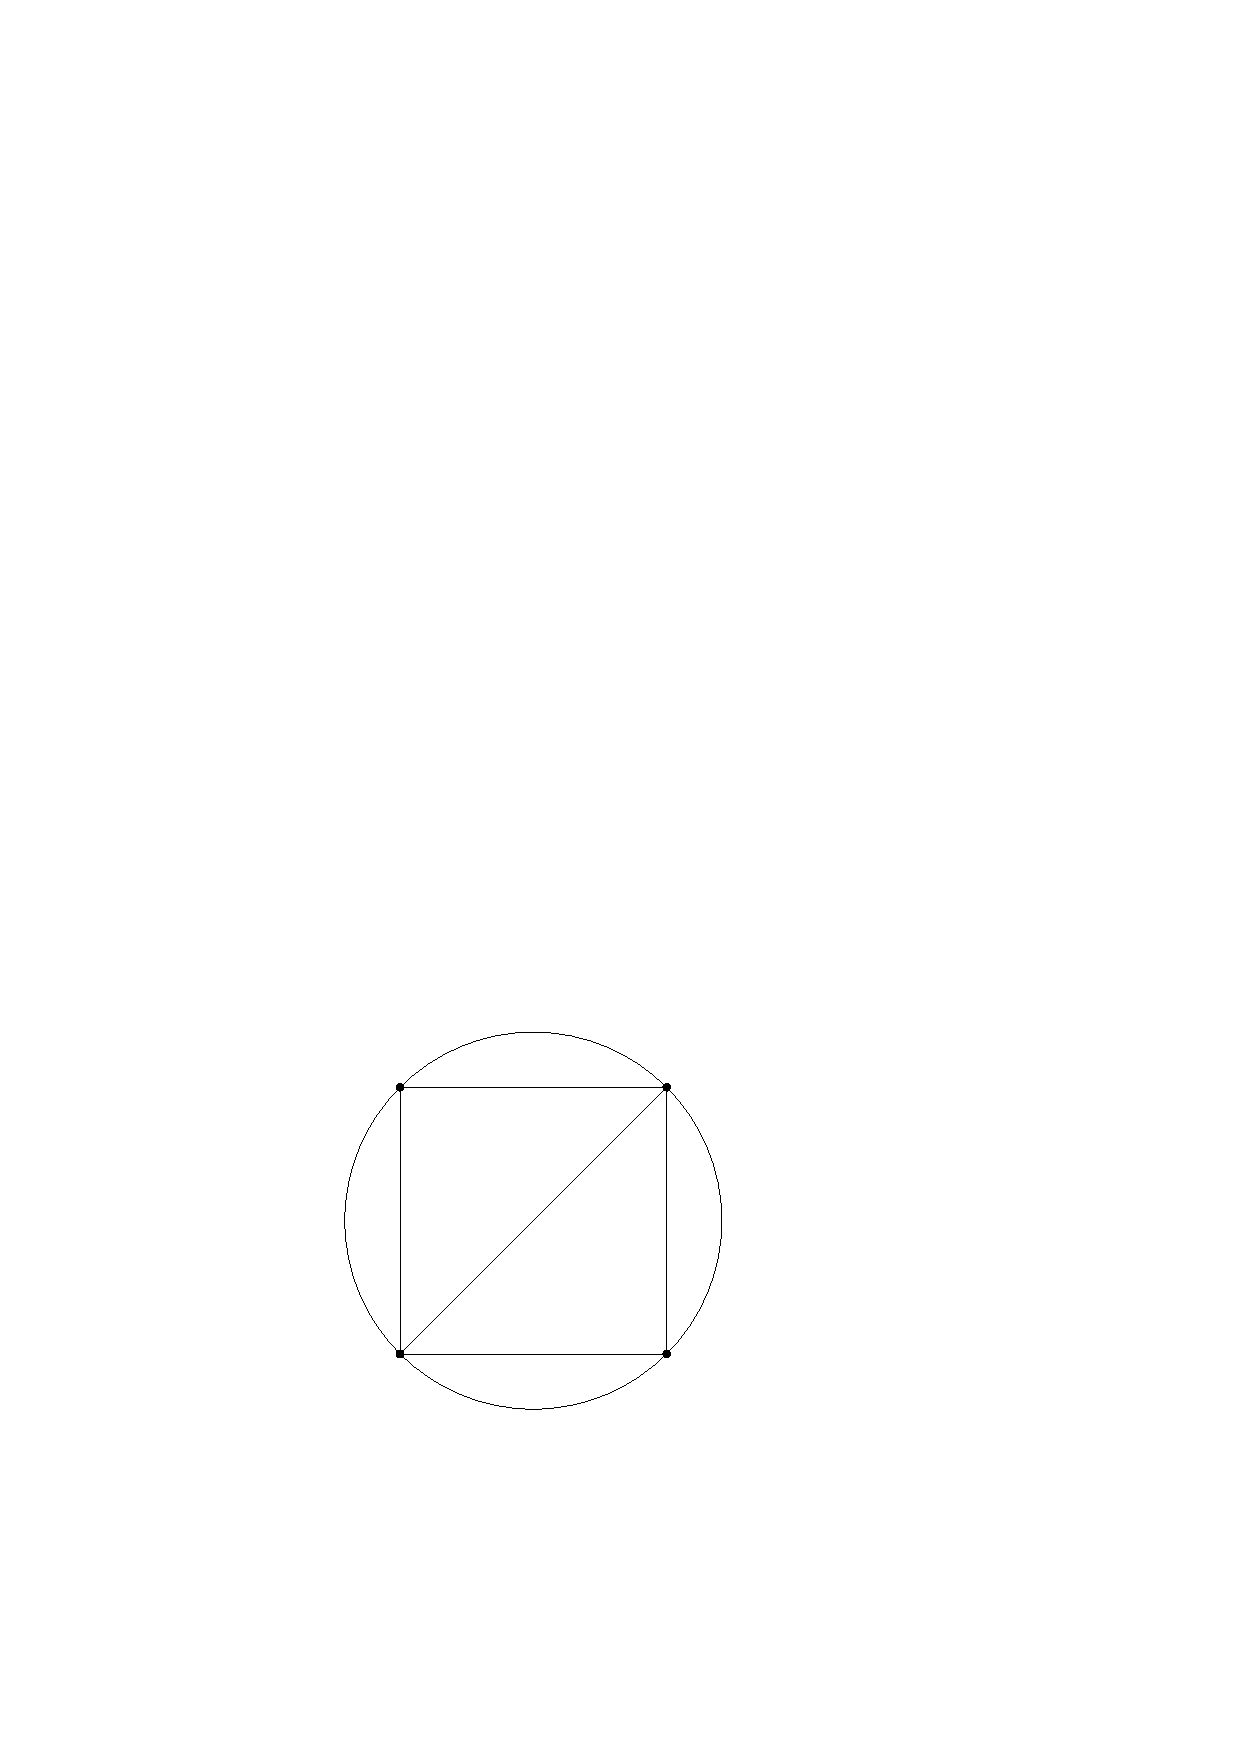
\includegraphics{images/non_general_pos_b.pdf}
    \end{subfigure}
    \caption{Possible triangulations in points in non general position}
    \label{fig:non_general_pos}
\end{figure}

There are many ways to compute delaunay triangulation of a point set. Most notably being the incremental construction and divide-and-conquer. We will talk about incremental construction as that is easier to understand and code. There are two methods for incremental construction

\subsection{Bowyer-Watson Algorithm}
Bowyer-Watson algorithm \cite{bowyer,watson} inserts points one by one in already existing delaunay triangulation. To insert point p, first all the triangles are collected whose circumcicles contain p. The set of triangles are deleted to create a cavity. This cavity is re-triangulated with the p as shown in Figure \ref{fig:bow_wat}. The algorithm to easily extensible to higher dimensions. In 3D, all tetrahedra are deleted whose circumspheres contain p forming a cavity. This cavity is then re-tetrahedralized to update the delaunay tetrahedralization. 

\begin{figure}[h]
    \centering
    \begin{subfigure}[t]{0.5\textwidth}
        \centering
        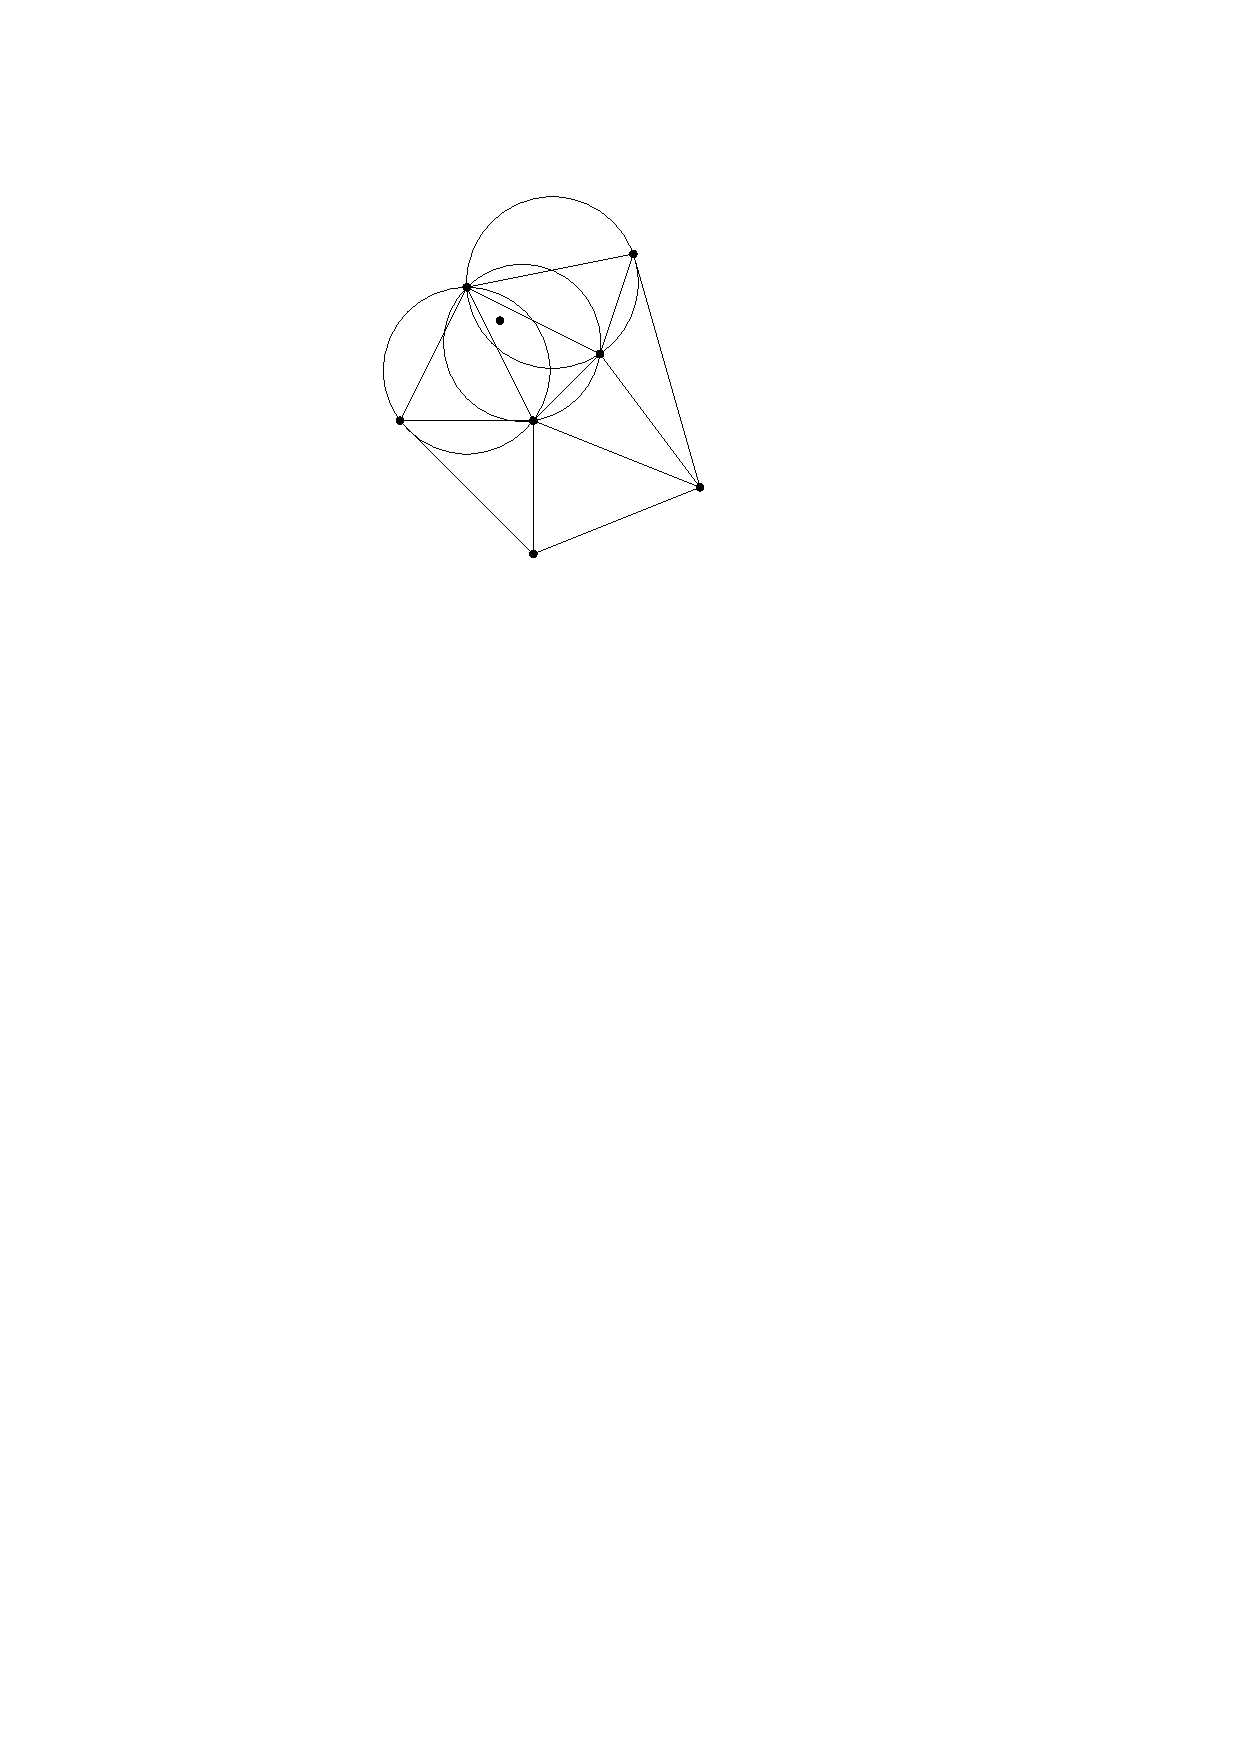
\includegraphics{images/bow_wat_a.pdf}
        \caption{all triangles whose circumcircles contain the new point are deleted}
    \end{subfigure}%
    \begin{subfigure}[t]{0.5\textwidth}
        \centering
        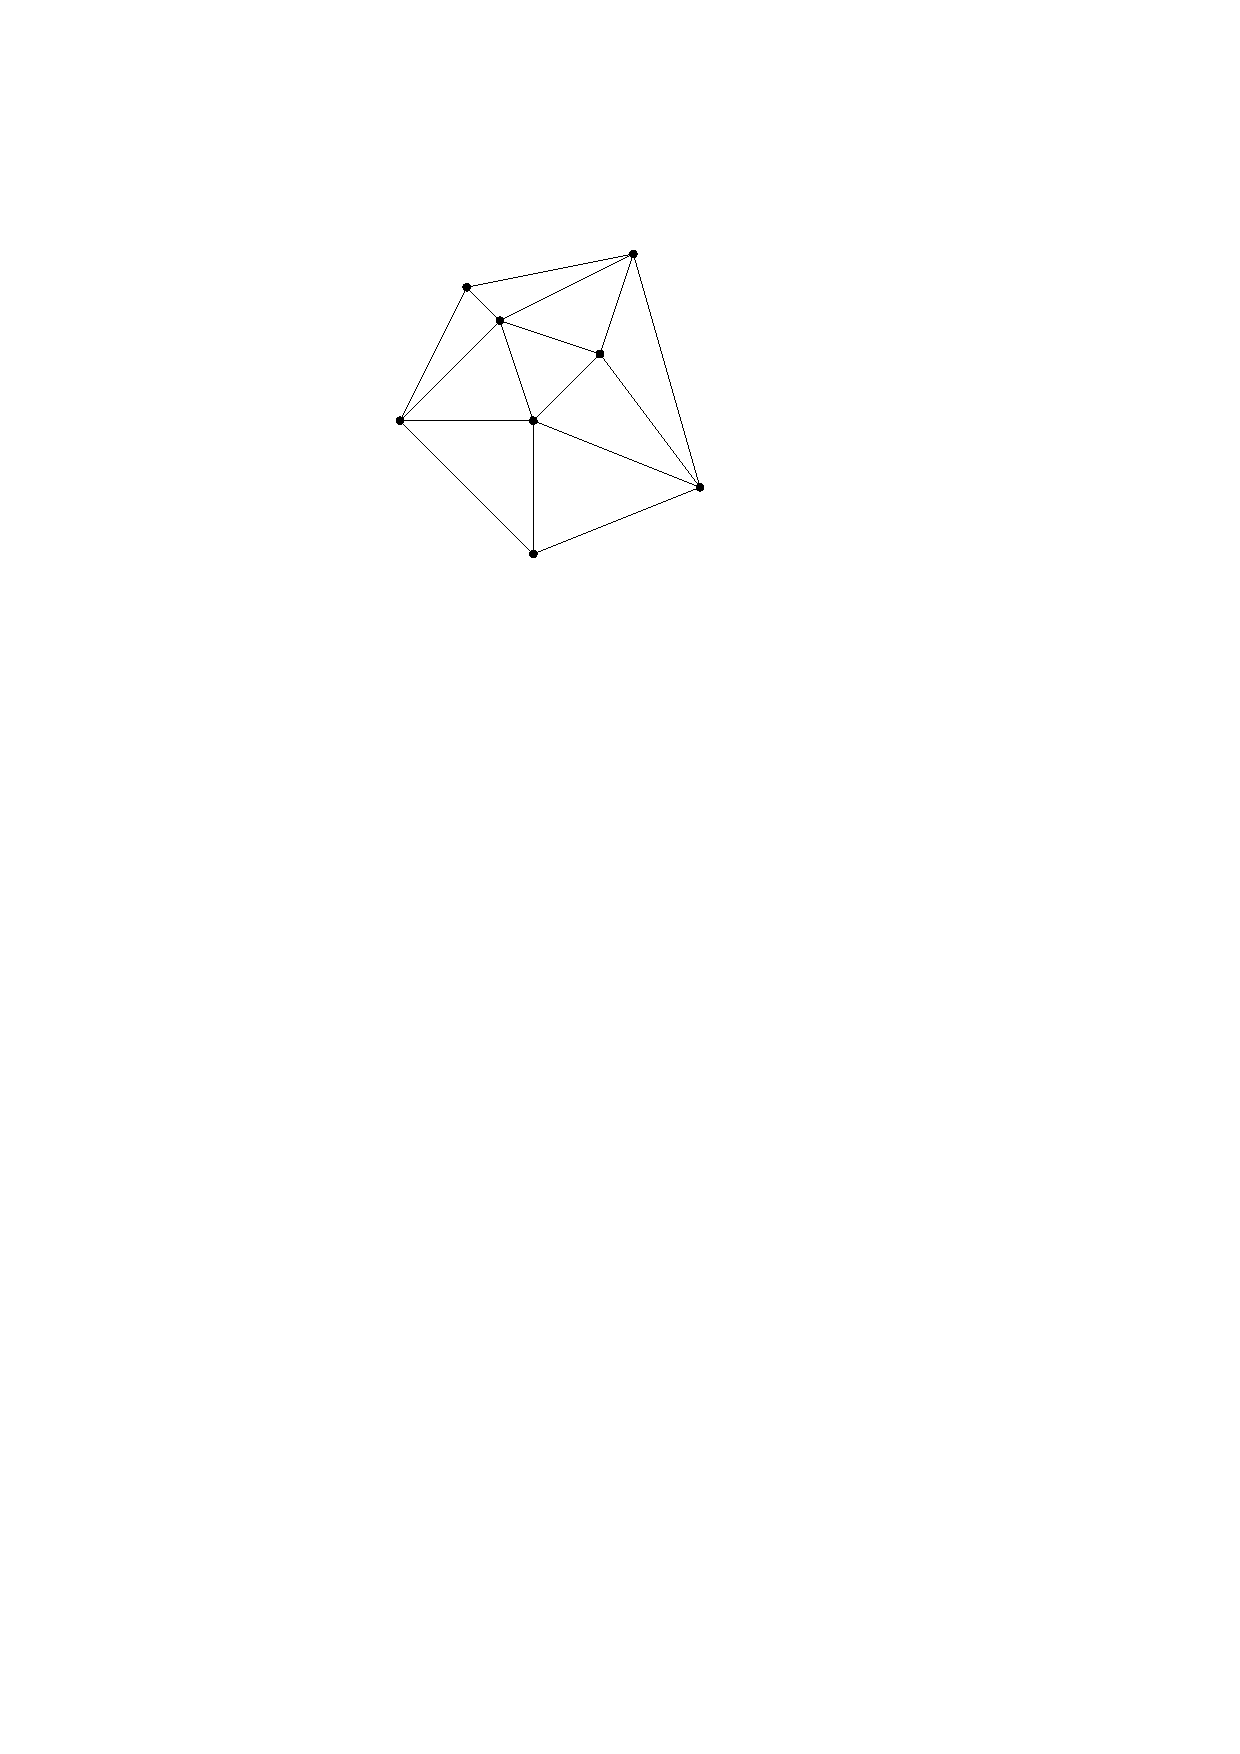
\includegraphics{images/bow_wat_b.pdf}
        \caption{updated triangulation with new point}
    \end{subfigure}
    \caption{Bowyer Watson Algorithm}
    \label{fig:bow_wat}
\end{figure}

It is fairy easy to implement but is prone to robustness issues if robust predicates are not used. If points are not in general position, then bowyer-watson algorithm can lead to invalid triangulation due to floating point round-off errors. This can lead to catastrophic program crashes and failures.

\subsection{Lawson flip Algorithm}
In 2D, the idea is to flip all non-delaunay edges in the triangulation. One can start with some arbitrary triangulation and then keep on flipping non-delaunay edges until all edges are delaunay. In incremental construction, a point p is inserted in following steps:
\begin{enumerate}
	\item First the triangle is found which contains the point p.
	\item Each edge of that triangle is connected to the point to form 3 new triangles. Old triangle is deleted.
	\item Apply flipping to all the non-delaunay edges starting from the new triangles going outwards till no non-delaunay edge is left.
\end{enumerate}

Theoretically,it can take $n^2$ flips, but in practice, it can be treated as constant. See Figure \ref{fig:law_flip} for flips in action.

\begin{figure}[h]
    \centering
    \begin{subfigure}[t]{0.5\textwidth}
        \centering
        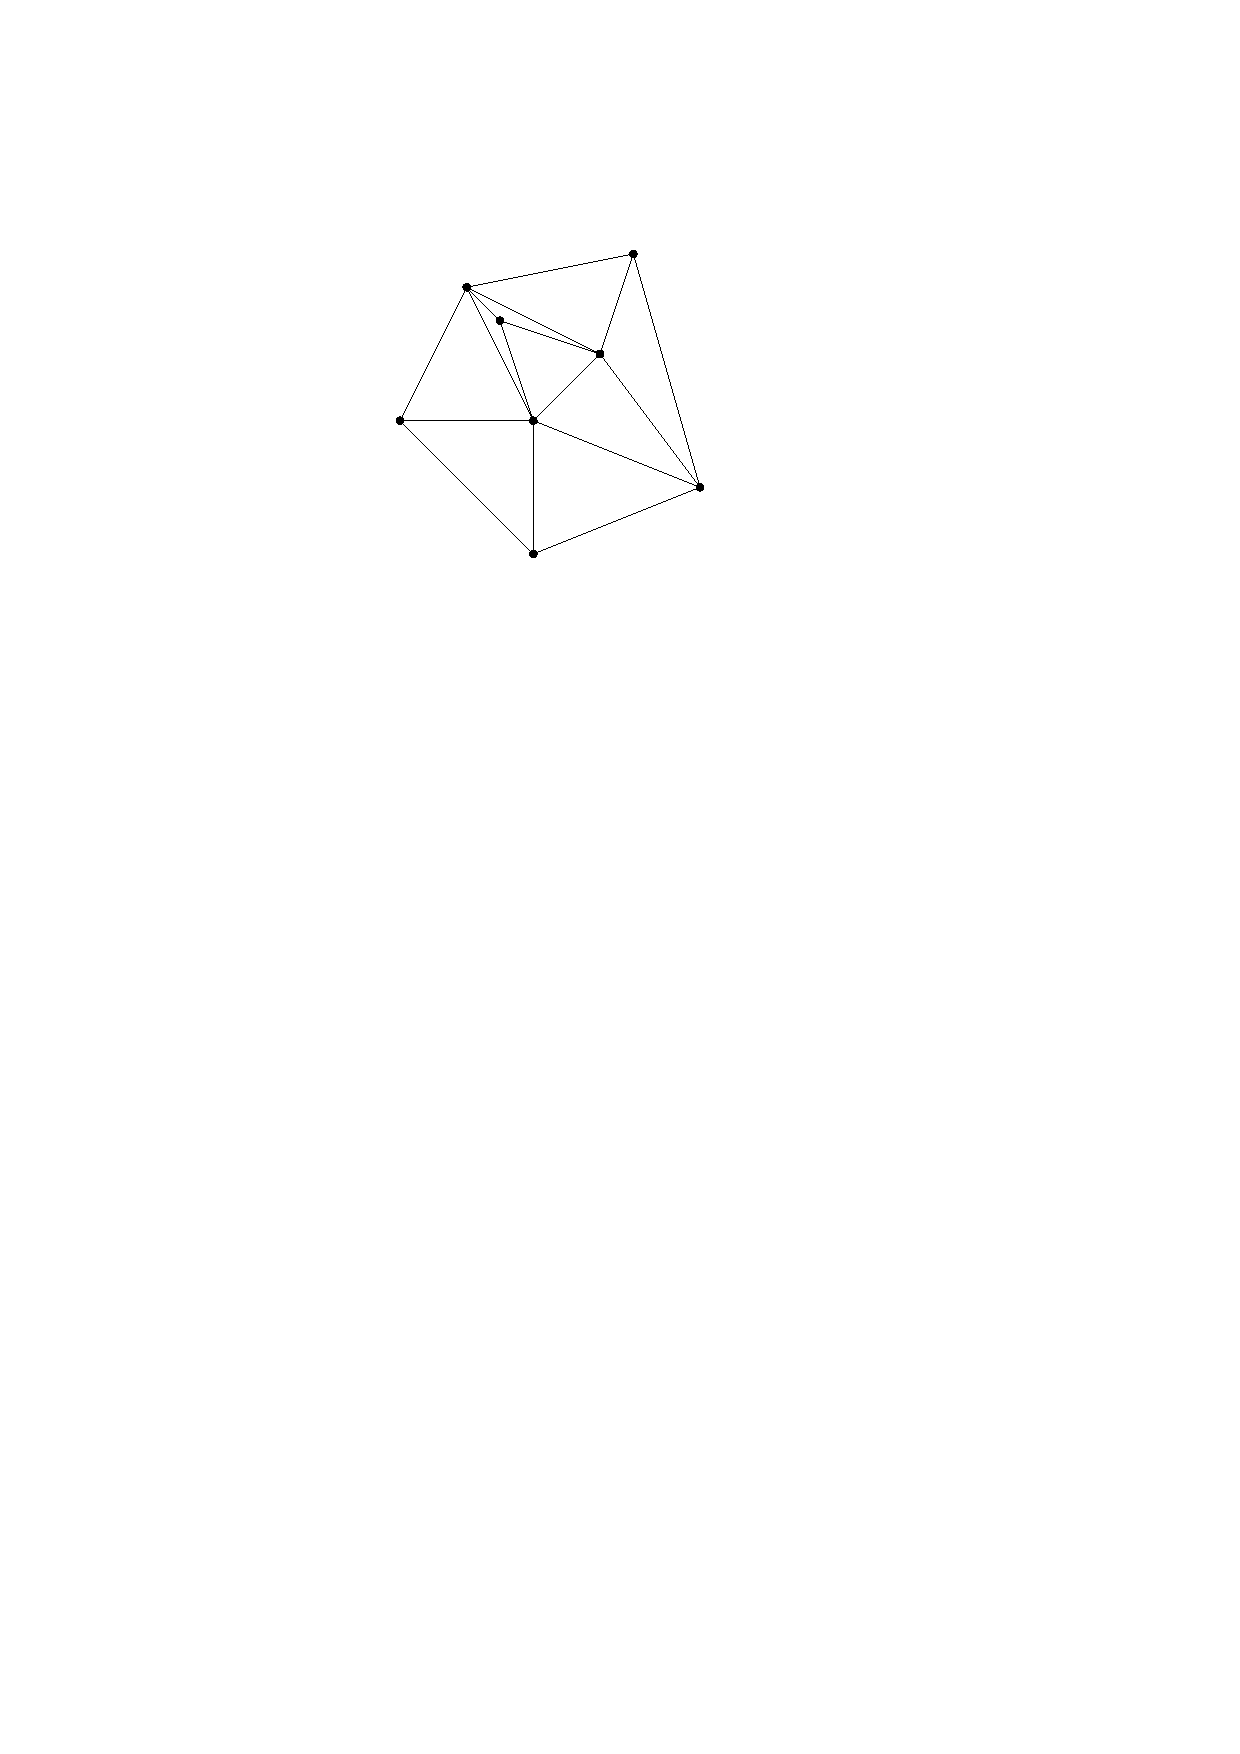
\includegraphics{images/law_flip_a.pdf}
        \caption{point is inserted in the triangle}
    \end{subfigure}%
    \begin{subfigure}[t]{0.5\textwidth}
        \centering
        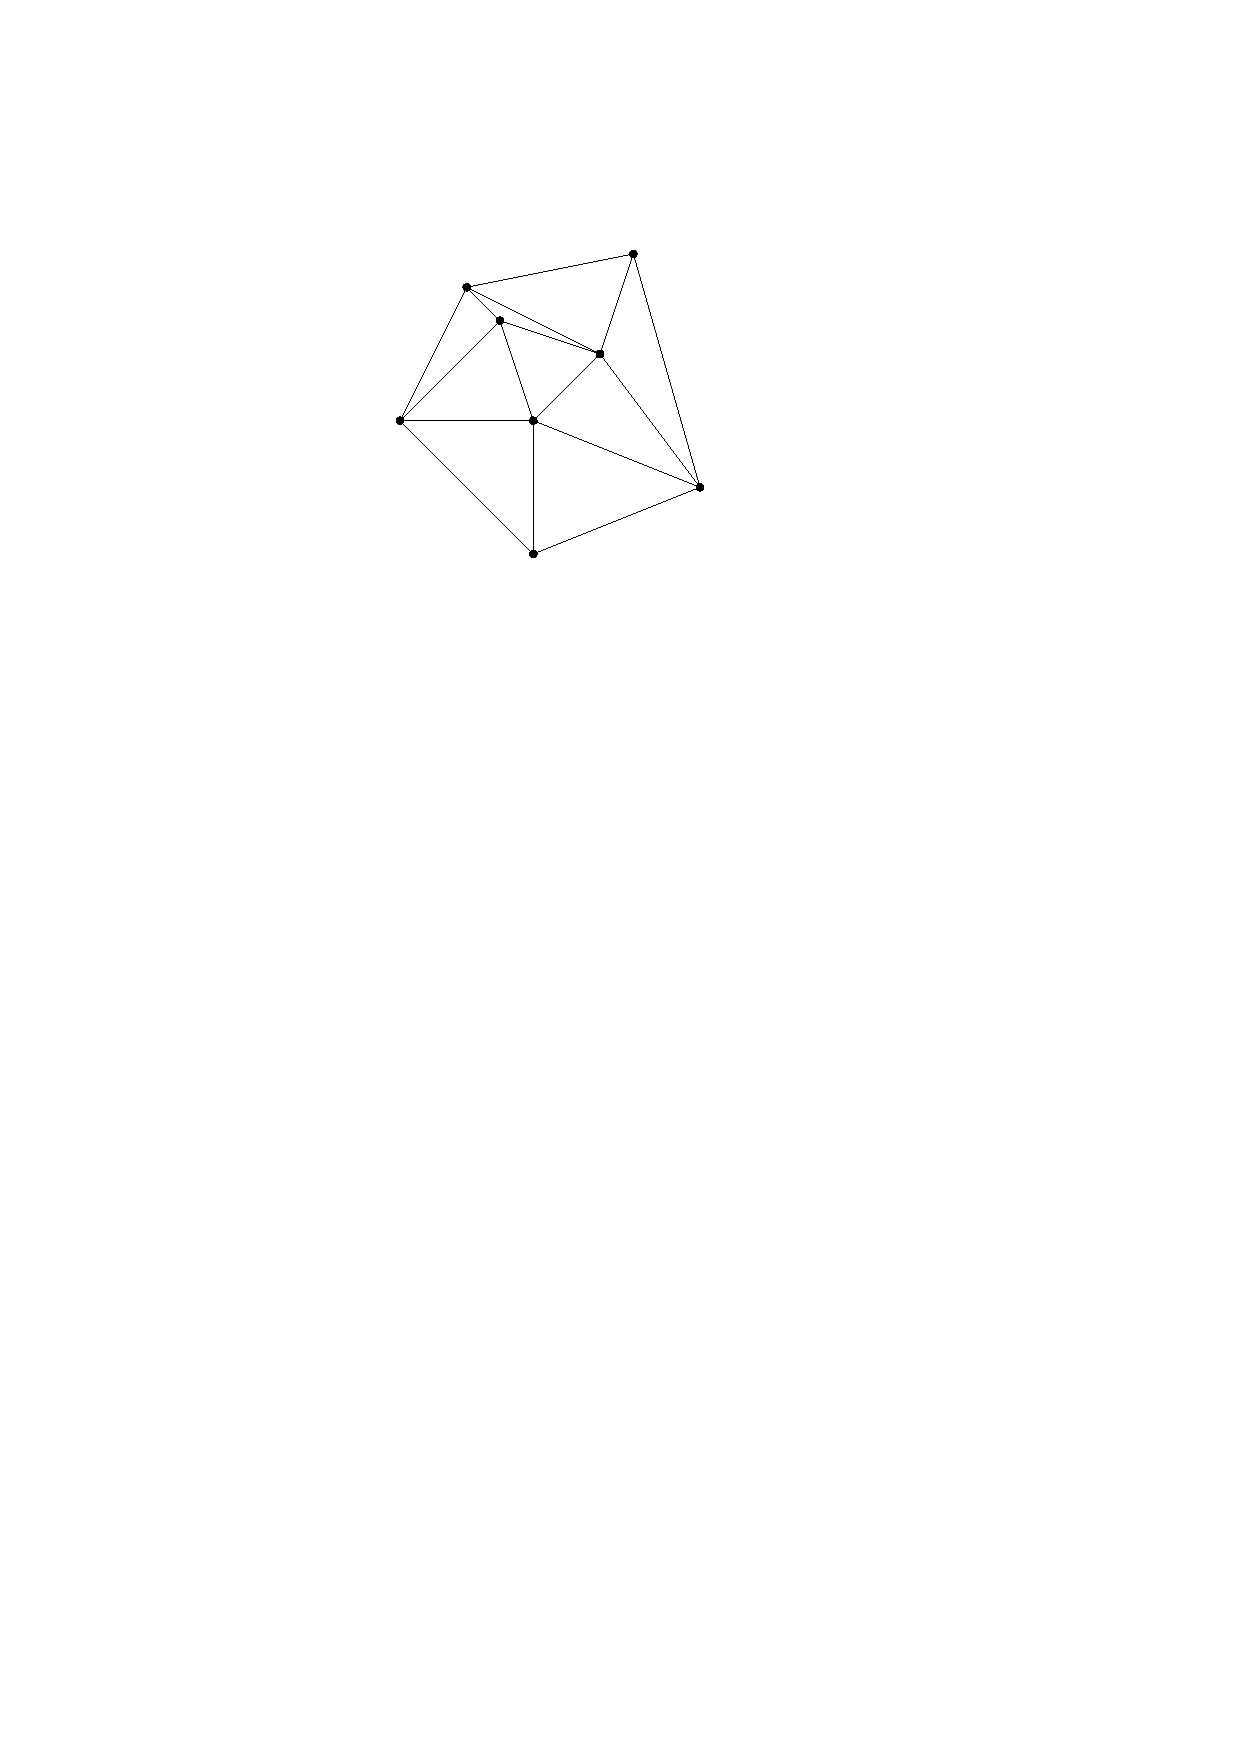
\includegraphics{images/law_flip_b.pdf}
        \caption{non-delaunay edge is flipped}
    \end{subfigure}
    
    \begin{subfigure}[t]{0.5\textwidth}
        \centering
        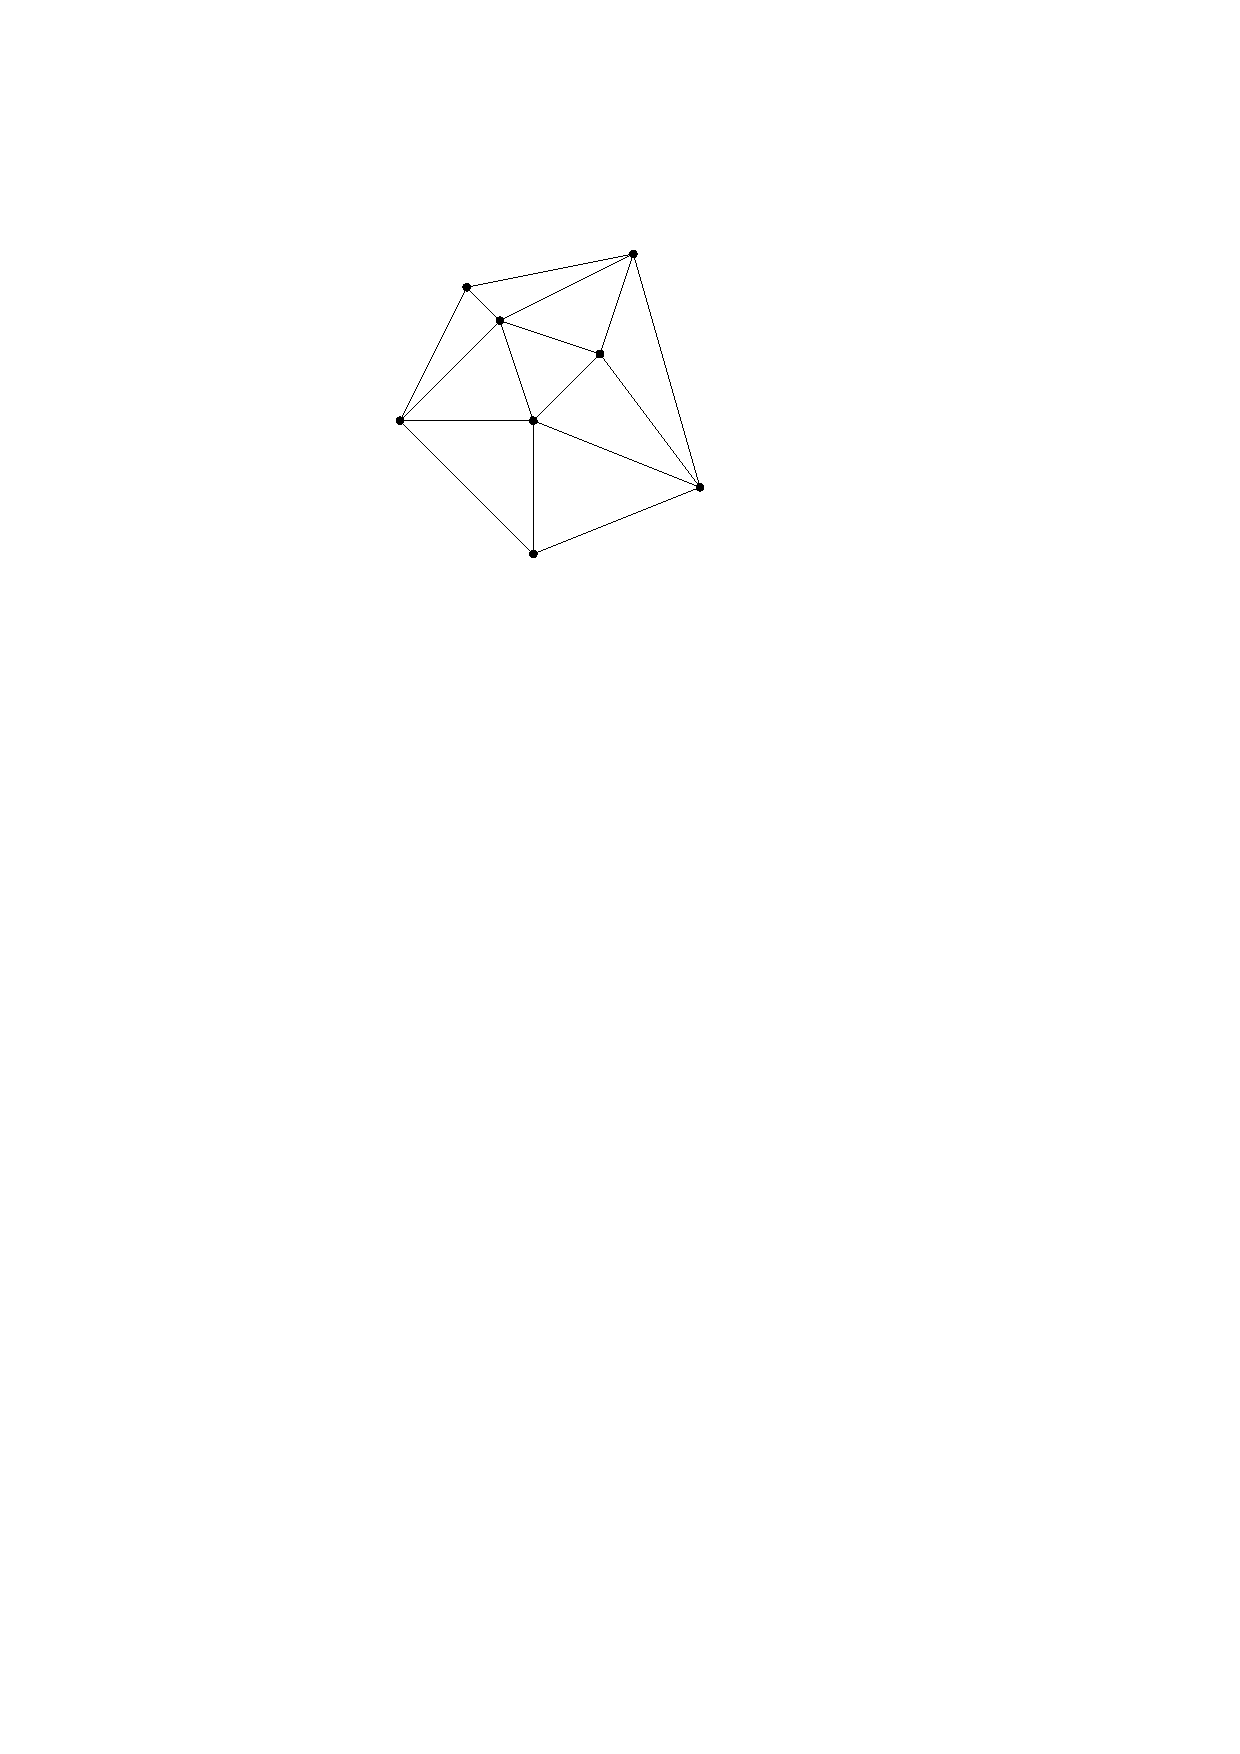
\includegraphics{images/law_flip_c.pdf}
        \caption{another non-delaunay edge is flipped and process stops as there are no more non-delaunay edges}   
    \end{subfigure} 
    \caption{Lawson Flip Algorithm}
    \label{fig:law_flip}
\end{figure}

This flipping \cite{lawson} technique is quite useful in smoothing. After relocating every vertex to new position, flipping is used to restore delaunayness.

Though the core of algorithm remains same in 3D but flipping is not straight forward in 3D as in 2D. In 3D, edges and faces both can be flipped. Unlike in 2D, not every non-delaunay configuration of edge/faces  can be flipped. There are two major flips in 3D \cite{joe}. 
\begin{enumerate}
	\item 1-4 flip : This is equivalent to inserting the point in a tetrahedra.
	\item 4-1 flip : This is equivalent to removing a point from the tetrahedra.

\begin{figure}[ht]
    \centering
    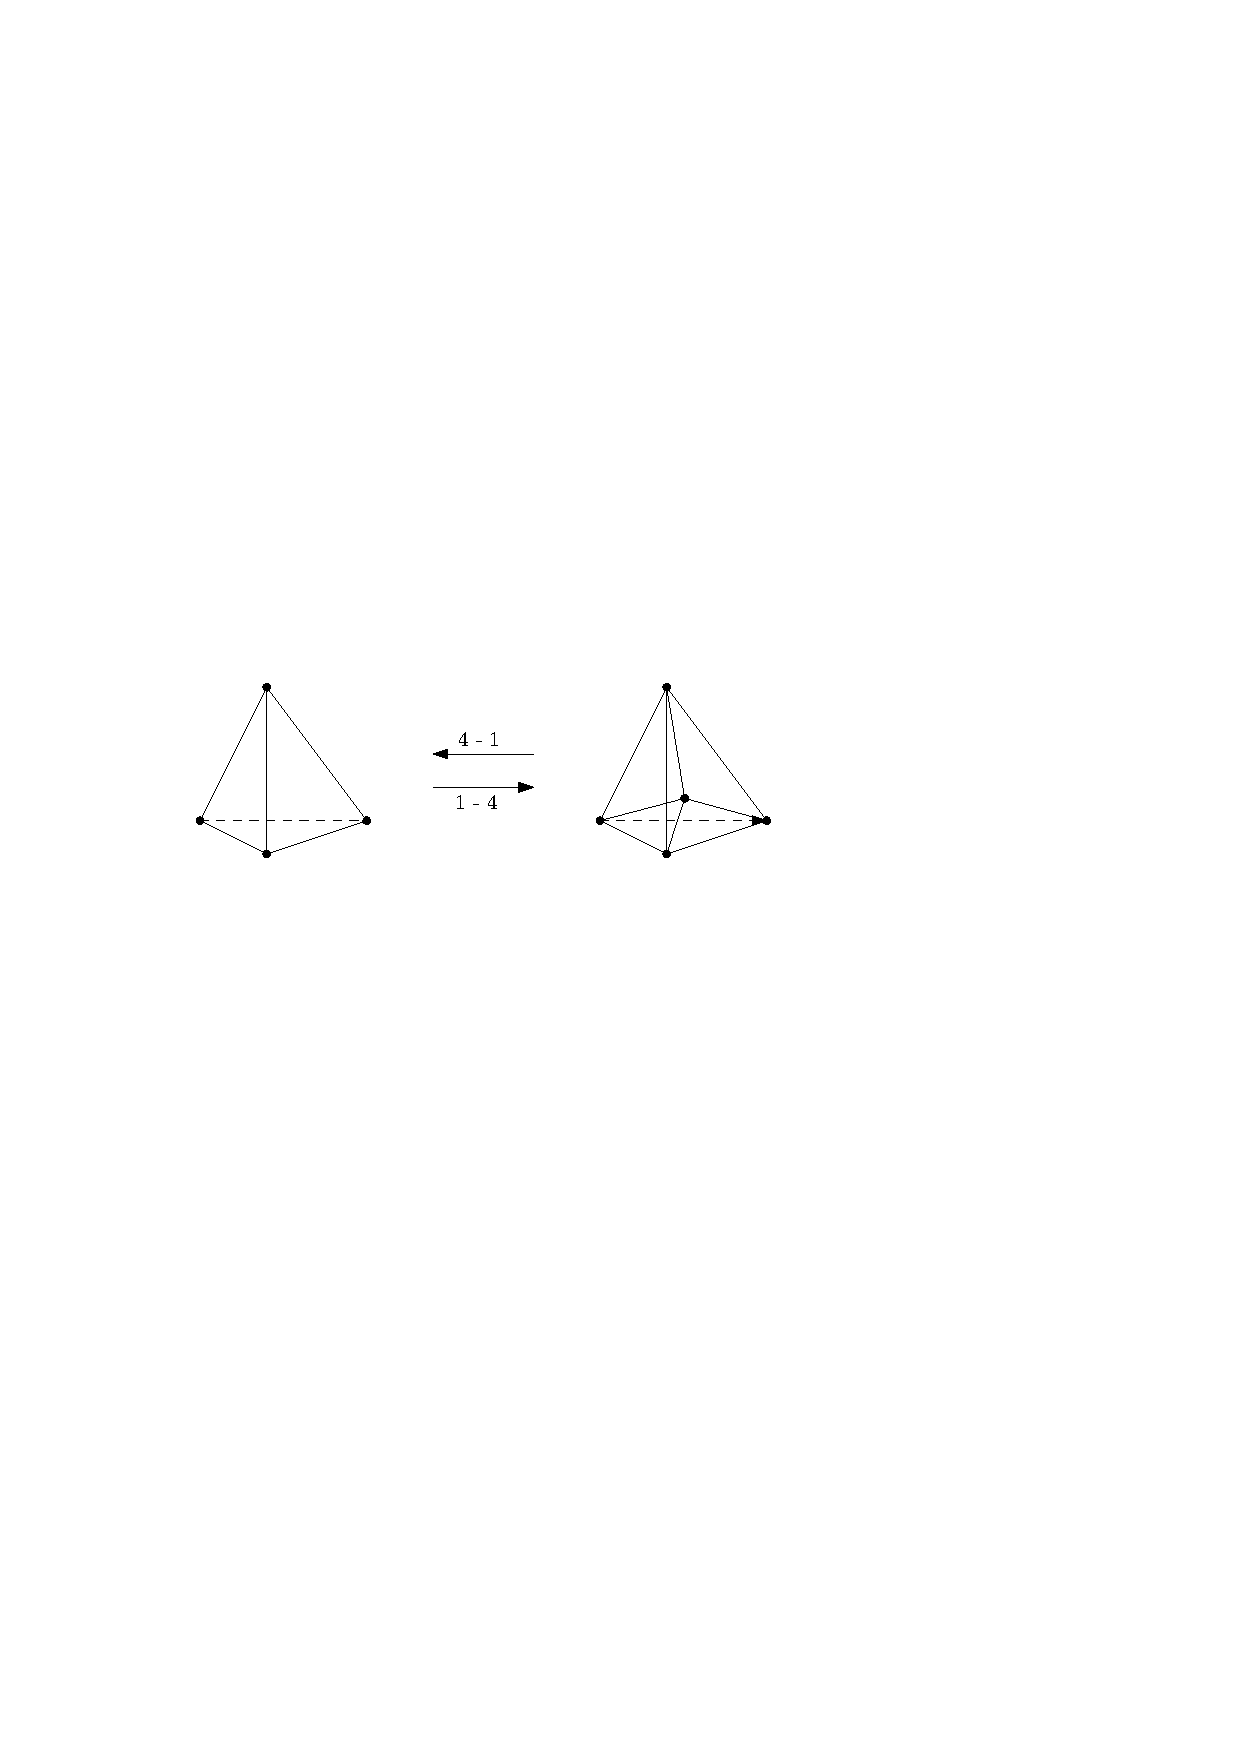
\includegraphics{images/1-4.pdf}
    \caption{1-4 flip}
    \label{fig:1_4_flip}
\end{figure}

Here 3 tetras are combined to create 2 tetras.
	\item 2-3 flip : A face is flipped only when it is part of 2 tetras and all points of 2 tetra lie on the convex hull formed by the tetras. So, 2 tetras are flipped to give 3 tetras.
	\item 3-2 flip : A edge is flipped only when it is part of 3 tetras.
Here 3 tetras are combined to create 2 tetras.

\begin{figure}[ht]
    \centering
    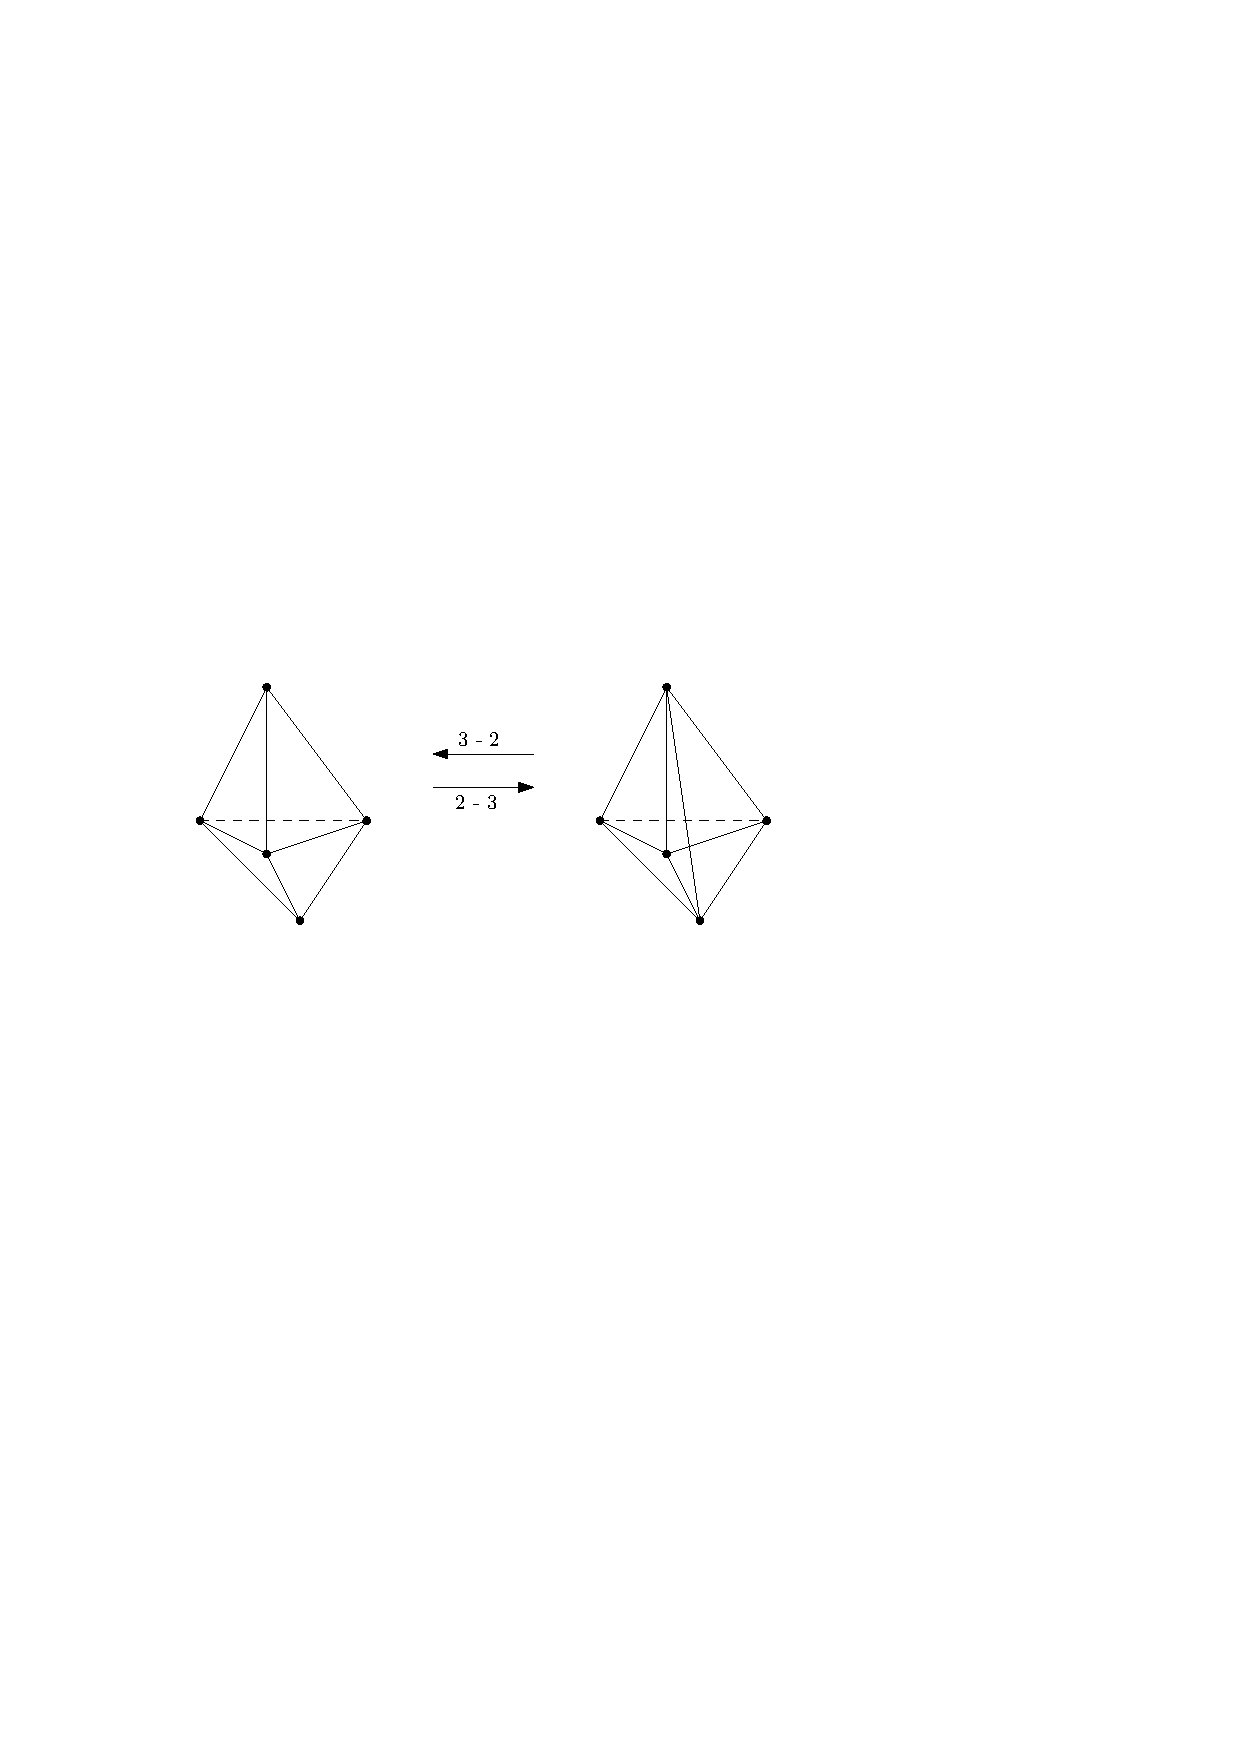
\includegraphics{images/2-3.pdf}
    \caption{2-3 flip}
    \label{fig:2_3_flip}
\end{figure}

\end{enumerate}

There are other flips also, 2-2 flip and 4-4 flip, which are useful in degenerate cases. If 4 tetra sharing an edge have degenerate points and 4 points are planar, then one of better configurations can be chosen. Same for 2-2 flip.

For performing flips after relocation of vertex to new point, flips are useful in 3D similar to 2D. Delaunay by flips has one major advantage over Bowyer-Watson that triangulation is always valid despite floating point errors. But in practice, flipping is slightly slower than former method.

\section{Smoothing Algorithms}
Laplacian smoothing is one of the most popular smoothing schemes. It comprises of all those algorithms \cite{dafield} which relocates the vertex to weighted average of all incident vertices. This works only for convex domains so for non-convex domains,extra check of validity of mesh is performed. But still it is faster than other more sophisticated methods. 
% formula
\begin{eqnarray}
x^*= \frac{1}{k} \sum_{x_j \in \Omega_i, x_j \neq x_i} x_j
\end{eqnarray}
% end formula
where $x*$ is the new location, $x_i$ is the vertex in consideration, $\Omega_i$ is the star of the vertex.

In practice, smoothing is iterative method and is performed until certain threshold value is reached or certain number of iterations are done. There are many methods to perform smoothing, in the following sections, we describe some of the popular smoothing methods in 2D. 

% section 3 : smoothing background, bit of history
% ODT, CVT, angle based, couple more
\subsection{Laplacian Smoothing}
In Laplacian smoothing, a vertex v is simply relocated to the centroid of the vertices connected to v. This centroid point can be treated as solution of spring torsion system. There is no guarantee for quality improvement and it might produce inverted elements. But it is simple and fast to implement and can give good results if number of iterations are less.
% formula and images

\subsection{Smart Laplacian Smoothing}
Shortcomings of laplacian is addressed in this one. Relocation strategy is same but before relocating any vertex, vertex is passed through checks to see if it improves the quality of neighborhood simplices, otherwise vertex's current position is not changed. So, there is an extra check for quality evaluation but still this method is inexpensive and avoids inverted elements \cite{freitag}.

\subsection{Angle Based Smoothing}
Angle based smoothing was given by Zhou and Shimada \cite{zhou&shimada} which tries to relocate the vertex to a position such that new position yields an optimum angle distribution on the angles formed by each side of the star.
% draw a figure for better explanation.
This method is computationally expensive than laplacian but offers better results and avoids creating inverted elements without extra checks. Finding optimum location is based on heuristics and notably there were two methods of finding new location due to Zhou and Shimada \cite{zhou&shimada}, Xu and Newman \cite{xu&newman}.

\subsection{Centroidal Voronoi Tessellation (CVT) Based Smoothing}
Centroidal Voronoi tessellation \cite{cvt} for a given point set is collection of voronoi cells such that each cell has centroid from the point set. CVT is applied in image analysis, flow control, dimension reduction etc. In mesh generation, CVT configuration of points provides an optimal distribution of points. CVT can be applied through LLoyd \cite{lloyd} iterations to initial delaunay triangulation to improve the mesh quality. In each Lloyd iteration, voronoi regions of each point p is calculated and p is relocated to centoid of the voronoi region given by 
% figure and formula
\begin{eqnarray}
x^*= \frac{1}{|\Omega_i|} \sum_{T_j \in \Omega_i} |T_j|C_j
\end{eqnarray}
% end formula
where  $x^*$ is the new location, $|\Omega_i|$ is the star of the point and $T_j$ is $j$th triangle of star, $|.|$ denotes the area in 2 dimension and $C_j$ is the circumcenter of $j$th triangle. There are other methods based on CVT, but Lloyd iterations are suitable for mesh smoothing despite its slow convergence.

\subsection{Optimal Delaunay Triangulation (ODT) Based Smoothing}
Delaunay triangulation minimizes the interpolation error for the function $|x|^2$ among all the triangulations for a given set of points. So, for the function $f(x) = |x|^2$, ODT is the triangulation with least error. Chen and Xu \cite{chen&xu} studied and proved that this definition can be used to devise an smoothing strategy. They found a unique solution to the interpolation error which results in new location as given by
% formula for new location	
\begin{eqnarray}
x^*=-\frac{1}{2|\Omega_i|} \sum_{T_j \in \Omega_i}(\nabla |T_j(x)| \sum_{x_k \in T_j, x_k \neq x_i} |x|^2)
\end{eqnarray}
% end formula
In the above equation $x^*$ is the new location, $|\Omega_i|$ is the star of the point and $T_j$ is $j$th triangle of star. Its convergence is slower than laplacian methods 




